\documentclass{WileyMSP-template}

\begin{document}

\pagestyle{fancy}
\rhead{\includegraphics[width=2.5cm]{vch-logo.png}}

\title{Teleoperation System with 6-DoF Haptic Feedback for Manipulation}

\maketitle

% Author: Please give full first and last names for authors and include * after the name of all corresponding authors

\author{Author One}
\author{Author Two}
\author{Author Three*}

% Dedication

\dedication{Optional dedication here. If no dedication is required, please leave blank}

% Affiliations: Please provide adacemic titles (Prof. or Dr.) for all authors where applicable, and include an institutional email address for all corresponding authors
\begin{affiliations}
A. N. Author, A. N. O. Author\\
Address\\
Email Address:

A. N. O. Author\\
Address

\end{affiliations}

% Keywords: Please provide a minimum of three and a maximum of seven keywords, separated by commas
\keywords{Teleperation, Haptic Feedback, Manipulation}

% Abstract should be written in the present tense and impersonal style (i.e., avoid we), and be at most 200 words long
\begin{abstract}

  Aerial manipulations using aerial robots are gaining attention for their work in high places and hazardous locations. 
  While autonomous control of robots has advanced, teleoperation by human operators is still necessary for tasks in complex and unknown environments. 
  In such teleoperation, haptic feedback that allows the operator to perceive the forces exerted on the robot is important. 
  In many cases, underactuated multirotors are used for teleoperation, but the use of fully actuated multirotors is advancing for more complex tasks. 
  Conventional teleoperation methods cannot achieve both intuitive control corresponding to the increased degrees of freedom and feedback of all 6-dimensional force and torque. 
  Therefore, in this study, we propose an operating device capable of expressing 6-dimensional force and torque, and a teleoperation system that makes it easy to perform work remotely using a fully actuated multi-rotor. 
  The operating device has a floating base with a thrust and vectoring mechanism, enabling independent control of position and attitude and independent presentation of forces and torques. 
  The teleoperation system has Position Mapping Mode and Velocity Mapping Mode settings, enabling both rapid movement in a wide area and precise movement for work. 
  We verified the effectiveness of the proposed method for aerial telemanipulations through experiments cleaning tilted walls. 
  Our new framework contributes to the realization of more complex aerial tasks using aerial robots.
  
\end{abstract}

% Text: Please use section headings and subheadings as specified below. For communications, all section headings apart from Experimental Section should be removed
% Please make the first reference to a display item bold: \textbf{Figure 1}
% Do not abbreviate Figure, Equation, etc.; display items are always singular, i.e., Figure 1 and 2.
% Equations are always singular, i.e., Equation 1 and 2, and should be inserted using the {equation} environment, not as graphics
% Please do not use footnotes in the text, additional information can be added to the Reference list.

%%%%%%%%%%%%%%%%%%%%%%%%%%%%%%%%%%%%%%%%%%%%%%%%%%%%%%%%%%%%%%%%%%%%%%%%%%%%%%%%
\section{Introduction}


%%%%%%%%%%%%%%%%%%%%%%%%%%%%%%%%%%%%%%%%%%%%%%%%%%%%%%%%%%%%%%%%%%%%%%%%%%%%%%%%
\section{Teleoperation Device}\label{sec:teleop_device}

\subsection{Design of Device}
The teleoperation device proposed in this research enables operators to perform tasks through remote robots easily.
Most tasks performed by humans require the use of some kind of tool.
Humans interact with the external environment through the handles of these tools and obtain information about the reaction forces.
Therefore, when performing tasks remotely, it is most intuitive to grip and operate the device as if the robot's tools were physically present in the operator's hands.

\begin{figure}[tb]
        \centering
        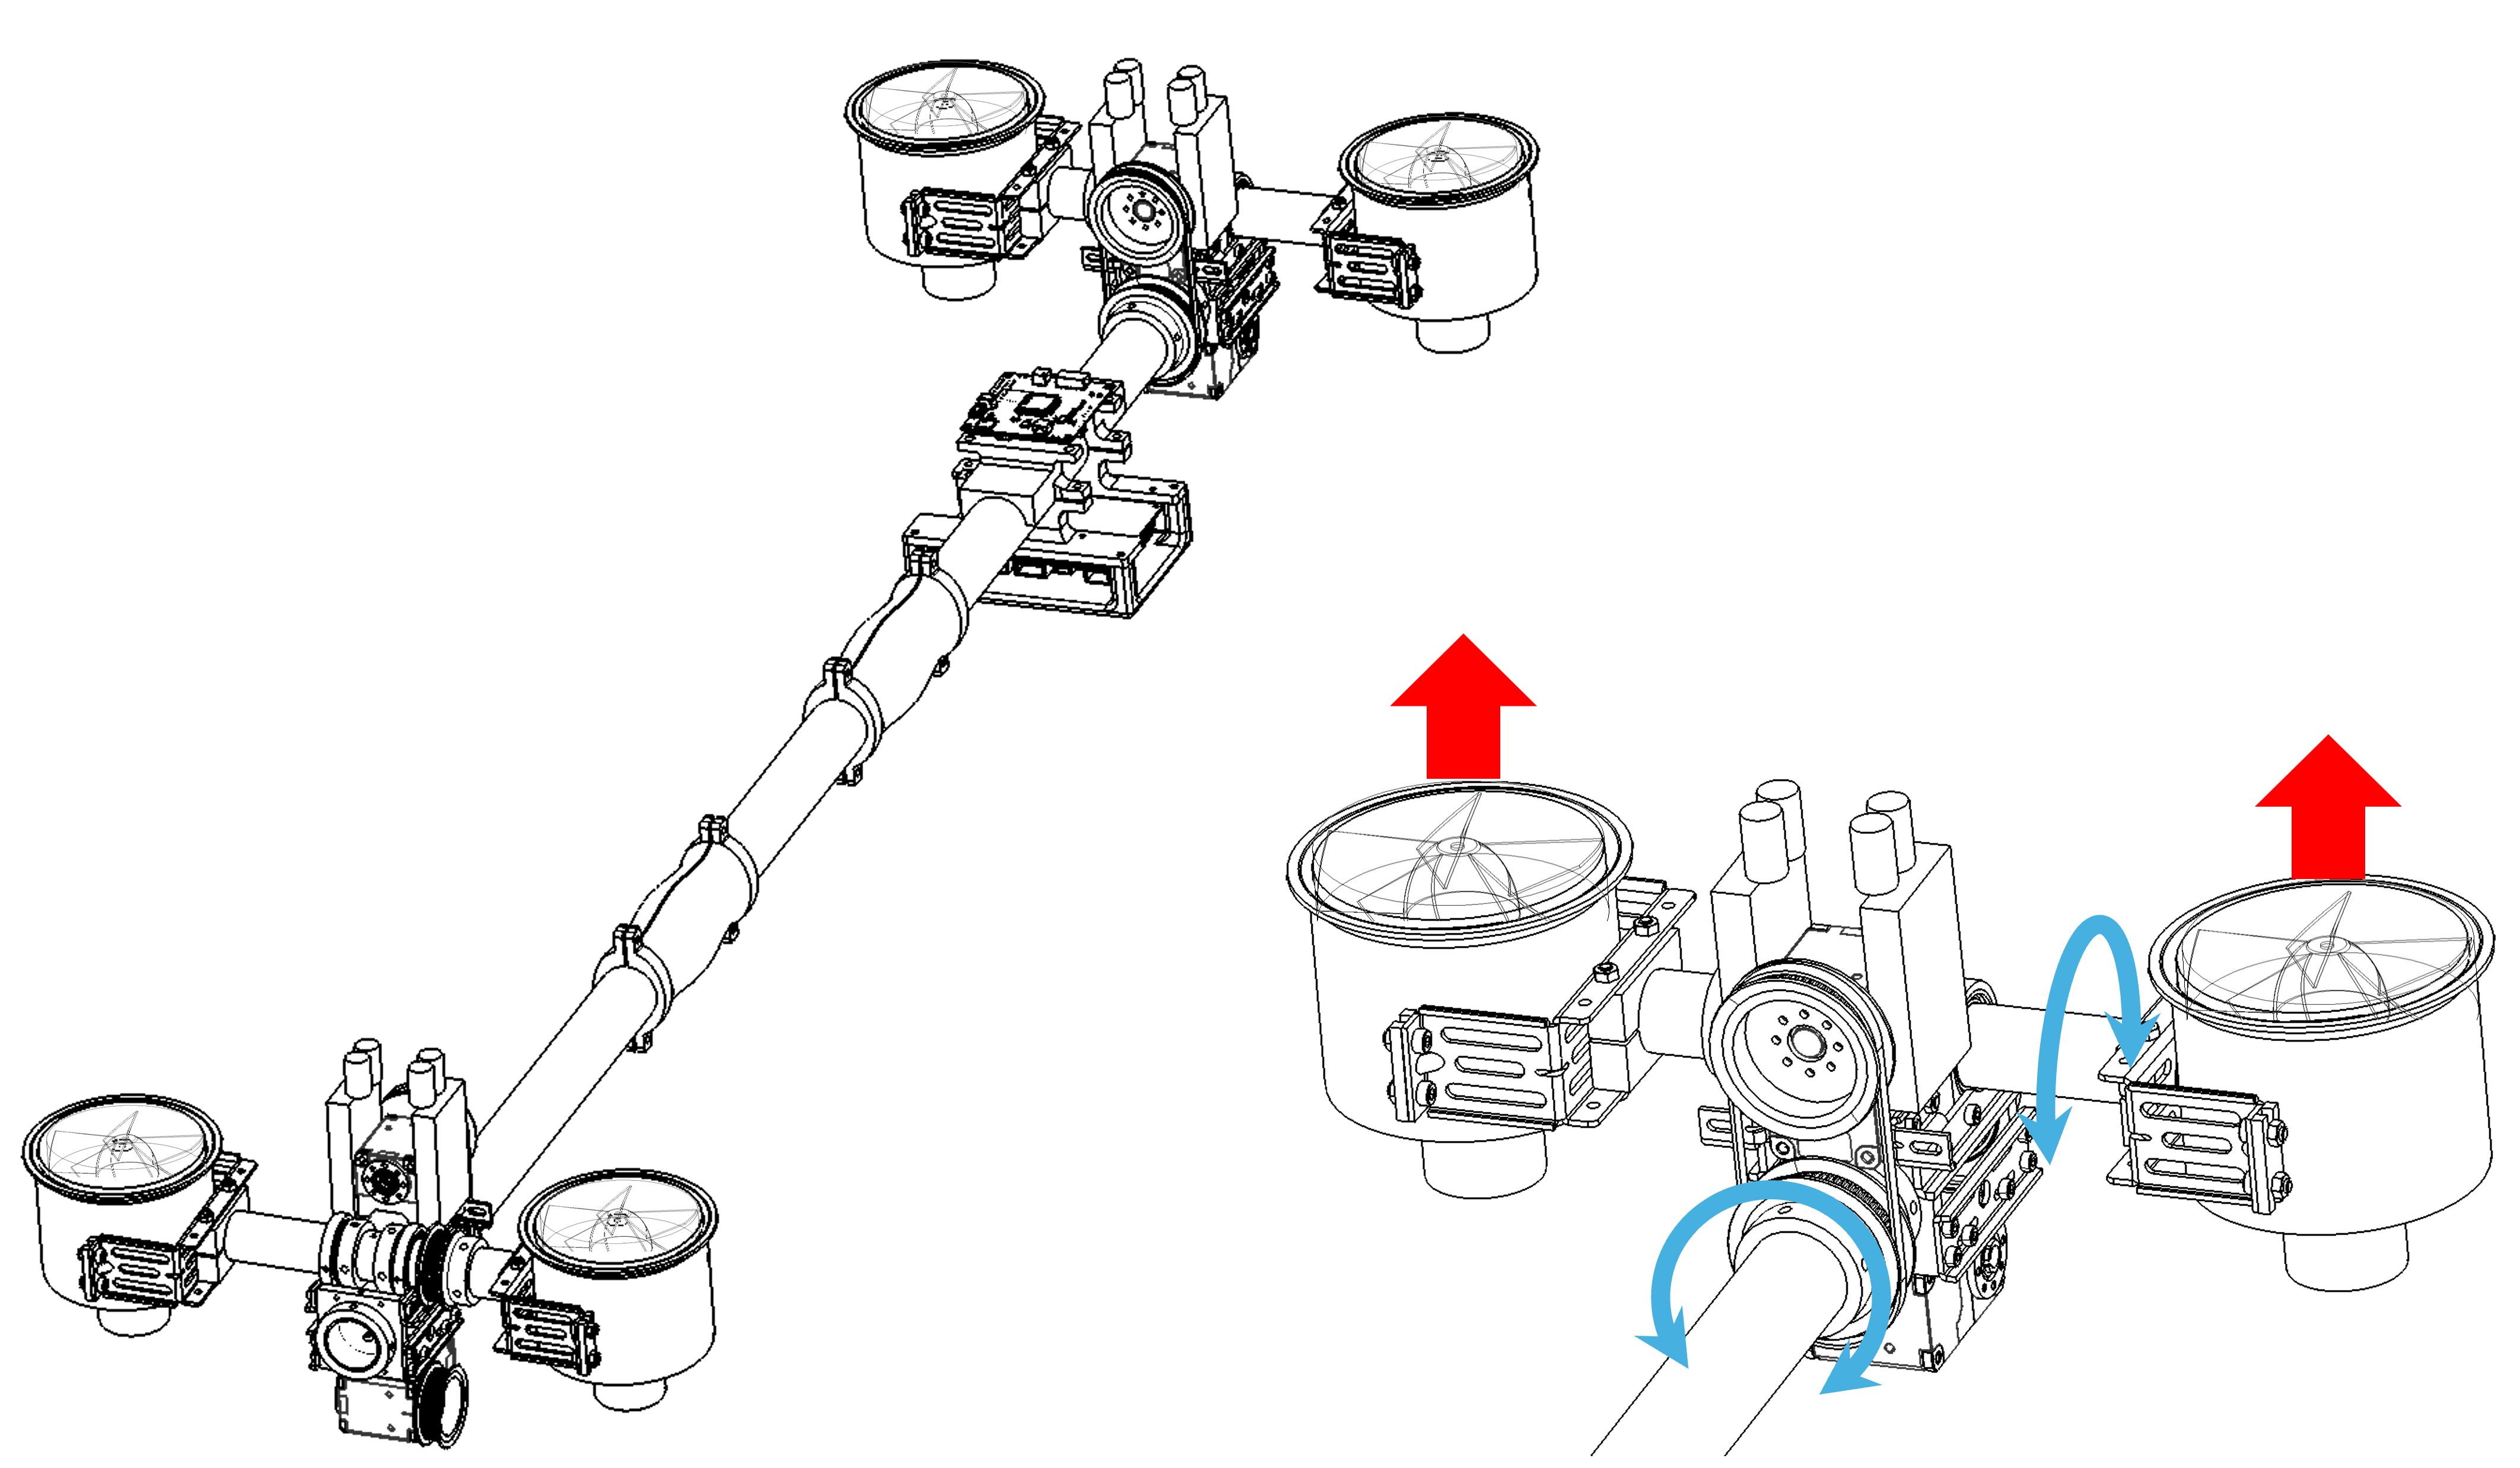
\includegraphics[width=0.9\columnwidth]{figs/device_design}
        \caption{Hardware design of proposed teleoperation device. Left:Whole view. Right:Thrust vectoring mechanism. The red arrows mean the thrust, and blue arrows is the rotational direction.}
        \label{fig:device_design}
\end{figure}

As mentioned in Sec. \ref{sec:intro}, in teleoperation using robots, the device must be capable of floating and independently providing 6-dimensional wrench.
To achieve these functions, we use thrust and a thrust vectoring mechanism.
The thrust vectoring mechanism is a modified version of the one proposed by Zhao et al \cite{DRAGON}.
As shown in the right of Fig. \ref{fig:device_design}, this thrust vectoring mechanism can rotate in 2 directions.
By attaching 2 rotors that generate thrust at both ends, it has a total of 4-DoF.
By attaching this module to both ends of a long rod modeled like a tool, the device as a whole can obtain 8-DoF for control input.
Since this is larger than the dimension 6 of the wrench we want to present, it allows us to present all wrenches with redundancy.

\subsection{Control of Device}

All of the following is considered in a coordinate system fixed to the device.
The DoF of control of this device are as shown on the top side of Fig. \ref{fig:control_line_graph}, but consider a virtual thrust as shown on the bottom side of Fig. \ref{fig:control_line_graph}.
The allocation matrix from virtual thrust to desired wrench can be expressed as 
\begin{equation}
        Q_1 = \left( \begin{array}{cc} I_3 & I_3 \\ skew(\bm{p}_{f_{{\text{v}}1}}) & skew(\bm{p}_{f_{{\text{v}}2}}) \end{array} \right) ,
\end{equation}
where $I_3 \in R^{3\times3}$ is identity matrix, $\bm{p}_{f_{{\text{v}}i}}$ is position vector of the virtual thrust $\bm{f}_{\text{v}i}$ point in the coordinate system of the handle, and $skew(\bm{p})$ is skew-symmetric matrix of $\bm{p}$.
The virtual thrust $\bm{f}_{\text{v}} = [\bm{f}_{\text{v}1}, \bm{f}_{\text{v}2}]^T$ is calculated from the desired wrench after removing torque around x-axis $\bm{W}_{\text{des}} = [F_{\text{des}x}, F_{\text{des}y}, F_{\text{des}z}, T_{\text{des}y}, T_{\text{des}z}]^T$ as follows.
\begin{equation}
        \bm{f}_{\text{v}} = Q_1^\# (\bm{W}_{\text{des}} + \bm{g}) ,
\end{equation}
where $\bm{g} = [0, 0, Mg, 0, 0]^T$ is the gravity term, which is the product of the mass of the device $M$ and the gravitational acceleration.
And $Q_1^\# \in R^{6\times5}$ is the pseudo-inverse of $Q_1$ with excluding the 4th row corresponding to torque around the x-axis.
The vectoring angles is calculated as follows:
\begin{equation}
        \theta_i = \arctan\left(- \frac{f_{\text{v}iy}}{f_{\text{v}iz}} \right) ,
\end{equation}
\begin{equation}
        \phi_i = \arctan\left( \frac{f_{\text{v}ix}}{-f_{\text{v}iy} \cdot \sin(\theta_i) + f_{\text{v}iz} \cdot \cos(\theta_i)} \right) .
\end{equation}
When moving the vectoring mechanism, the following counter torque occurs around the x-axis.
\begin{equation}
        \tau_{\text{counter}} = \sum I_i \ddot{\theta_i} ,
\end{equation}
where $I_i$ is the ineria of the vectoring module around x-axis.

\begin{figure}[tb]
        \centering
        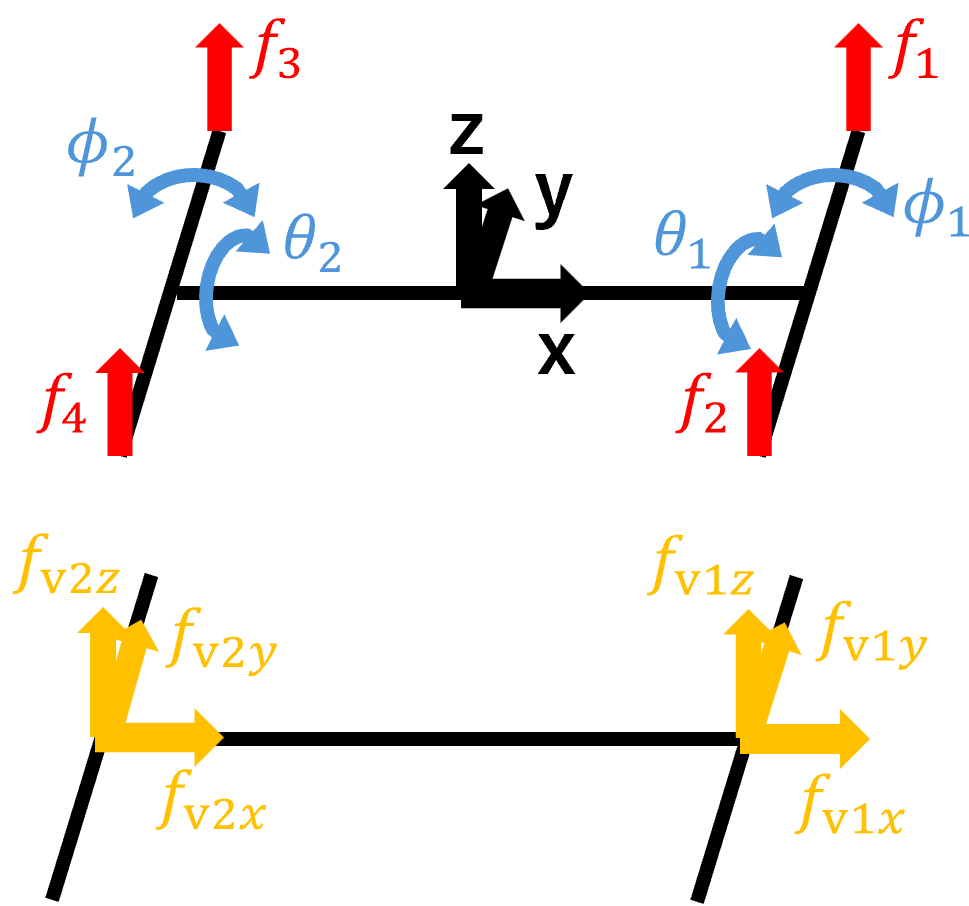
\includegraphics[width=0.7\columnwidth]{figs/control_line_graph}
        \caption{Top:Control DoF of the proposed device. The black allows shows the hadle coordinate system fixed on the device. Bottom:Virtual thrust considered on a control model.}
        \label{fig:control_line_graph}
\end{figure}

The allocation matrix from virtual thrust and torque around x-axis to the actual thrust can be expressed as
\begin{equation}
        Q_2 = \left( \begin{array}{cccc} 1 & 0 & 1 & 0 \\ 0 & 1 & 0 & 1 \\ d_1\cos\psi_1 & -d_2\cos\psi_2 & d_3\cos\psi_1 & -d_4\cos\psi_2 \end{array} \right) ,
\end{equation}
where $d_1, d_2, d_3, d_4$ is the distance from each rotor to the longitudinal axis of the device.
Then, the actual thrust $\bm{f} = [f_1, f_2, f_3, f_4]^T$ is calculated as follows:
\begin{equation}
        \bm{f} = Q_2^\# \begin{bmatrix} |\bm{f}_{\text{v}1}| \\ |\bm{f}_{\text{v}2}| \\ T_{\text{des}x} + \tau_{\text{counter}} \end{bmatrix} ,
\end{equation}
where $Q_2^\# \in R^{4\times3}$ is the pseuso-inverse of $Q_2$.
Since the range of force that can be exerted by the rotor is limited, the solution obtained here is not always feasible.
If the solution is outside the feasible range, substitute the closest feasible value and recalculate the solution.

%%%%%%%%%%%%%%%%%%%%%%%%%%%%%%%%%%%%%%%%%%%%%%%%%%%%%%%%%%%%%%%%%%%%%%%%%%%%%%%%
\section{Teleoperation System}
This chapter describes a teleoperation system for performing tasks using a remote robot.
The system consists of generating position and attitude commands from the operator to the robot, and generating wrench feedback from the robot to the operator.

\subsection{Position and Atiitude Operating Command}
Two main functions are required to control the position and attitude of a remote robot.
One is long-distance movement, which is the function of quickly moving within the wide area.
The other is precise movement, which is a function for performing detailed tasks accurately.
To achieve both of these functions, we developed two operating modes: Position Mapping Mode and Velocity Mapping Mode.

\subsubsection{Position Mappng Mode}
We propose Position Mapping Mode for precise tasks.
In this mode, the target position $\bm{p}_{\text{target}}(t)$ and quaternion $\bm{q}_{\text{target}}(t)$ is generated as follows:
\begin{equation}
        \bm{p}_{\text{target}}(t) = \bm{p}_{\text{robot}}(t_0) + \bm{k}_1 \odot (\bm{p}_{\text{device}}(t) - \bm{p}_{\text{device}}(t_0)) ,
\end{equation}
\begin{equation}
        \bm{q}_{\text{target}}(t) = \bm{q}_{\text{device}}(t) ,
\end{equation}
where $t_0$ refers to the moment of entering this mode, and $\odot$ is the Hadamard product, which is the product of each element of the vector.
And $\bm{k}_1$ is a scaling parameter that can be adjusted as appropriate depending on the task type.

\subsubsection{Velocity Mappng Mode}
On the other hand, we propose Velocity Mapping Mode for long-distance movement.
In this mode, the target velocity $\dot{\bm{p}}_{\text{target}}(t)$ and angular velocity $\dot{\bm{q}}_{\text{target}}(i)$ is generated as follows:
\begin{equation}
        \dot{\bm{p}}_{\text{target}}(t) = \bm{k}_2 \odot (\bm{p}_{\text{device}}(t) - \bm{p}_{\text{device}}(t_0)) ,
\end{equation}
\begin{equation}
        \dot{\bm{q}}_{\text{target}}(t) = \bm{k}_3 \odot (\bm{q}_{\text{device}}(t) - \bm{q}_{\text{device}}(t_0)) ,
\end{equation}
where $\bm{k}_2$ and $\bm{k}_3$ are scaling parameters.
Adding the amount of change in the device to the robot's position and quaternion at each time point is equivalent to controlling the robot's velocity.

In this mode, it is important for the operator to recognize the initial origin of the device, as well as when operating with a joystick. 
The device proposed in this study enables the operator to recognize the origin by providing a reaction wrench corresponding to the amount of movement from the origin of the device.
If the magnitude of the feedback wrench is made proportional to the amount of device movement, as with commands and control, the wrench near the origin becomes small, making it easy to lose sight of the origin.
Therefore, logarithmic conversion is used as follows:
\begin{equation}
        \bm{f}_{\text{feedback}} = \log (\bm{k}_4 \odot (\bm{p}_{\text{device}}(t) - \bm{p}_{\text{device}}(t_0))) ,
\end{equation}
\begin{equation}
        \bm{\tau}_{\text{feedback}} = \log (\bm{k}_5 \odot (\bm{q}_{\text{device}}(t) - \bm{q}_{\text{device}}(t_0))) ,
\end{equation}
where $\bm{k}_4$ and $\bm{k}_5$ are scaling parameters.
This conversion increases the feedback wrench near the origin, making it easier to recognize the origin.
In addition, in order to reduce the difficulty of operation, Stop Zone where no commands are sent to the robot is set near the origin.

By using these two modes appropriately, it is possible to perform tasks quickly and precisely in a large workspace.

\subsection{Wrench Feedback from Robot}


%%%%%%%%%%%%%%%%%%%%%%%%%%%%%%%%%%%%%%%%%%%%%%%%%%%%%%%%%%%%%%%%%%%%%%%%%%%%%%%%
% Experimental section
\section{Experimental Section}
\threesubsection{First part of experimental section}\\
\threesubsection{Second part of experimental section}\\


\medskip
\textbf{Supporting Information} \par %Please delete the Suppporting Information statement if it is not applicable. Please supply Supporting Information in another file. Supporting information should not be provided in .tex format
Supporting Information is available from the Wiley Online Library or from the author.

% Acknowledgements
\medskip
\textbf{Acknowledgements} \par %delete if not applicable))
Please insert your acknowledgements here

% References
\medskip

% Use the following code if you wish to generate your bibliography with BibTeX;
% replace the string "MSP-template" below with the name(s) of
% the BibTeX data base(s) you want to use.
% The resulting bibliography-output (the content of the .bbl file)
% must be pasted back into this file before submission.
% Please also include your BibTeX data base file(s) in your submission
% so that we can re-run BibTeX if necessary.
%
%\bibliographystyle{MSP}
%\bibliography{MSP-template}

\textbf{References}\\
\bibliographystyle{unsrt}
\bibliography{bib}

% 1	((Journal articles)) a) A. B. Author 1, C. D. Author 2, Adv. Mater. 2006, 18, 1; b) A. Author 1, B. Author 2, Adv. Funct. Mater. 2006, 16, 1.\\
% 2	((Work accepted)) A. B. Author 1, C. D. Author 2, Macromol. Rapid Commun., DOI: 10.1002/marc.DOI.\\
% 3	((Books)) H. R. Allcock, Introduction to Materials Chemistry, Wiley, Hoboken, NJ, USA 2008.\\
% 4	((Edited books or proceedings volumes)) J. W. Grate, G. C. Frye, in Sensors Update, Vol. 2 (Eds: H. Baltes, W. Göpel, J. Hesse), Wiley-VCH, Weinheim, Germany 1996, Ch. 2.\\
% 5	((Presentation at a conference, proceeding not published)) Author, presented at Abbrev. Conf. Title, Location of Conference, Date of Conference ((Month, Year)).\\
% 6	((Thesis)) Author, Degree Thesis, University (location if not obvious), Month, Year.\\
% 7	((Patents)) a) A. B. Author 1, C. D. Author 2 (Company), Country Patent Number, Year; b) W. Lehmann, H. Rinke (Bayer AG) Ger. 838217, 1952.\\
% 8	((Website)) Author, Short description or title, URL, accessed: Month, Year.\\
% 9	…((Please include all authors, and do not use “et al.”))\\

\end{document}
